\chapter{Example Chapter}
\label{example}
%In diesem Kapitel beschreiben Sie Ihren eigenen Beitrag
%- Es muss klar sein, worin die eigentliche Innovation besteht#

This chapter gives you some examples how to include graphics, create tables, or include code listings. But first, we start with a short description how you can efficiently cite in \LaTeX. The following footnote shows you how to reference URLs and where this document is available online.\footnote{\url{http://www.ovgu.de/tthuem}}

\section{Acronyms}

This template makes advantage of the glossaries package to support acronyms. The first occurence of an acronym is replaced by its definition, e.g., \gls{IDE}. All other occurences are replaced by the acronym (\gls{IDE}). The glossaries package also supports plural---\glspl{IDE}.

\glsreset{IDE}
Sometimes you want to make sure, that the long version is used, even if \gls{IDE} was inserted before.

\section{Citation}

There are several types of literature. The most citations are workshop and conference papers. Please use the inproceedings-tag for those citations, e.g.~\cite{KAK:GPCE09}. You should have short-hands for workshop and conference names to be sure the naming is consistent and uniform (see our BibTeX files how to do that).

Slightly different are articles published in journals, e.g.~\cite{KG:SME06}. Make sure you that the volume and number-tags are present and that no inproceeding is tagged as article or vice versa.

You might want to take a look at the example BibTeX file to find out how to cite books~\cite{CE:BOOK00}, technical reports~\cite{KCHNP:TR90}, websites~\cite{Coq:website}, PhD theses, or master theses~\cite{B:PHD03,R:MT09}.

\section{Formulas}

There are different types of mathematical environments to set formulas. The equation $E=m\cdot c^2$ is an inline formula. But you can also have formulas at a separate line (see \vref{eq:ex}).

	\begin{equation}\label{eq:ex}
			P=\bigl(\mathcal{A}\pimplies(\mathcal{B}\pequals\mathcal{C})\pand(\mathcal{B}\pequals\mathcal{D})\bigr)\pand(\mathcal{B}\pimplies\mathcal{A})\pand(\mathcal{C}\pimplies\mathcal{A})\pand(\mathcal{D}\pimplies\mathcal{A})
	\end{equation}

If you need multiple lines that are aligned to each other, you might want to use the following code.

	\newcommand{\fG}{\mbox{GraphLibrary}}
	\newcommand{\fE}{\mbox{Edges}}
	\newcommand{\fA}{\mbox{Algorithms}}
	\newcommand{\fD}{\mbox{Directed}}
	\newcommand{\fU}{\mbox{Undirected}}
	\newcommand{\fN}{\mbox{Number}}
	\newcommand{\fC}{\mbox{Cycle}}
	\begin{eqnarray*}
	&& \fG\\
	&\pand& (\fG \pimplies \fE) \pand (\fE \por \fA \pimplies \fG)\\
	&\pand& (\fE \pequals \fD \por \fU) \pand (\pnot \fD \por \pnot \fU)\\
	&\pand& (\fA \pequals \fN \por \fC)\\
	&\pand& (\fC \pimplies \fD).\\
	\end{eqnarray*}

\section{Graphics}

In \vref{fig:ex}, we give a small example how to insert and reference a figure.

\begin{figure}[htbp]
	\centering
		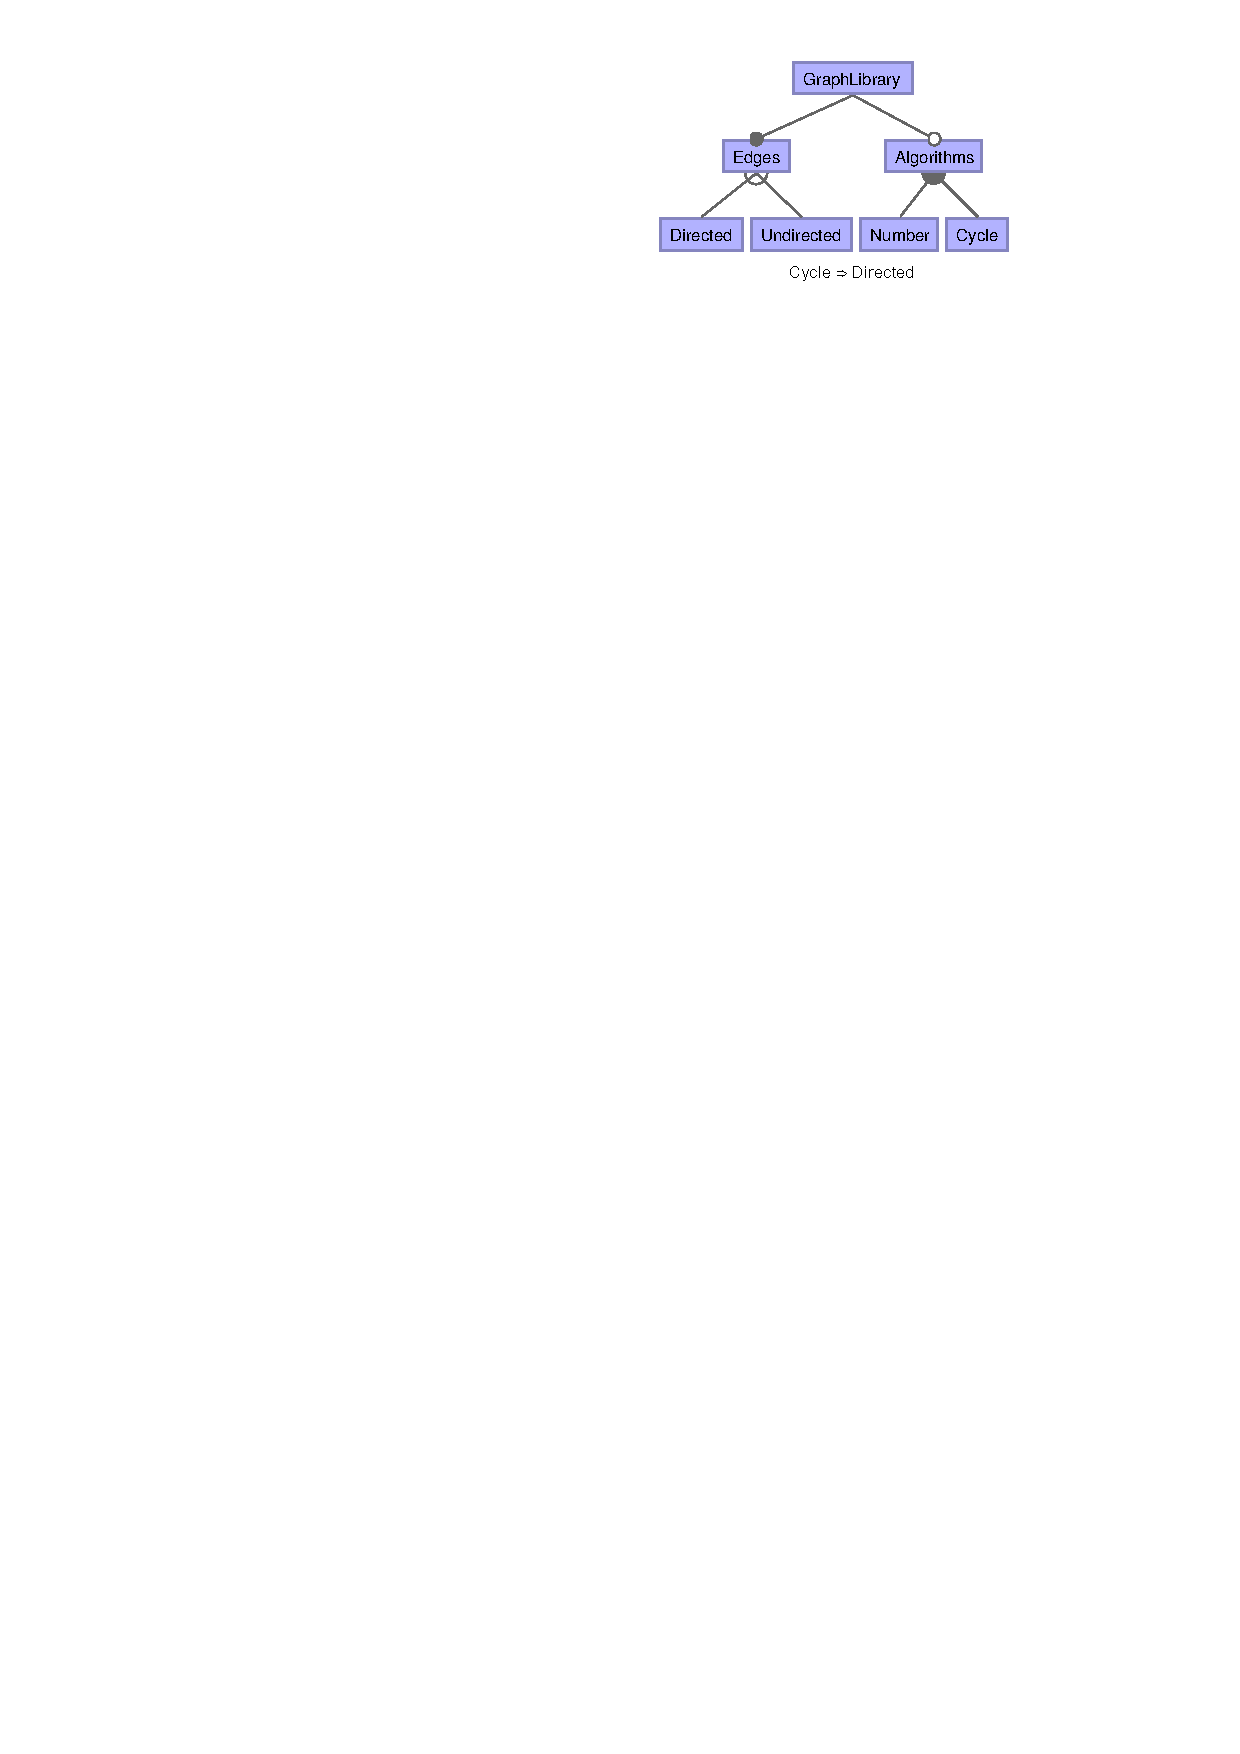
\includegraphics[scale=1.25]{example}
	\caption{A Feature Model Representing a Graph Product Line}
	\label{fig:ex}
\end{figure}

\section{Tables}

\vref{tab:ex} shows the result of a simple tabular environment.

\begin{table}[htbp]
	\centering
		\begin{tabular}{cc}\toprule
			Group Type & Propositional Formula\\\midrule
			And & $(P \pimplies C_{k_1} \wedge\ldots\wedge C_{k_m}) \pand (C_1\vee\ldots\vee C_n \pimplies P)$\\\addlinespace
			Or & $P \pequals C_1\vee\ldots\vee C_n$\\\addlinespace
			Alternative & $(P \pequals C_1\vee\ldots\vee C_n) \pand \mbox{atmost}1(C_1,\ldots,C_n)$\\
			\bottomrule
		\end{tabular}
	\caption{Mapping a Feature Model to a Propositional Formula}
	\label{tab:ex}
\end{table}

\section{Code Listings}

In \vref{lst:ex}, we give an example of a source code listing. 

\begin{lstlisting}[style=Java,float=htb,caption={Java Source Code},label={lst:ex}]
class A extends Object {
	A() { super(); }
}
class B extends Object {
	B() { super(); }
}
class Pair extends Object {
	Object fst;
	Object snd;
	Pair(Object fst, Object snd) {
		super(); this.fst=fst; this.snd=snd;
	}
	Pair setfst(Object newfst) {
		return new Pair(newfst, this.snd);
	}
}
\end{lstlisting}
